\documentclass[11pt,twoside]{article}
\usepackage[spanish, es-tabla]{babel}
\usepackage[utf8]{inputenc}
\usepackage{booktabs}
\usepackage{booktabs}     % tablas 
\usepackage{tabulary}     % tablas
\usepackage{graphicx}      % poner imagenes 
\usepackage{float}         % para fijar las imagenes con h y H
\usepackage{fancyhdr}
% Margins
\topmargin 0.02cm
\headheight 0.02cm
\textwidth 15.50cm
\oddsidemargin .0in
\evensidemargin .0in

\date{}

\begin{document}

\fancypagestyle{firststyle}
{
	\fancyhead[R]{ \tiny{Facultad de Ciencias, Facultad de Minas \\
	Universidad Nacional de Colombia, Sede Medellín\\
	2018}}
	\fancyhead[L]{}
	\fancyfoot[LO,RE]{}
	\fancyfoot[LE,RO]{ \vspace{10pt}\thepage}
	\renewcommand{\headrulewidth}{0pt}
	\renewcommand{\footrulewidth}{0pt}
}

\thispagestyle{firststyle}
\begin{center}
\Large{{\bf COLNALYTICS\\
\vspace{20pt}   PREDICCIÓN DEL REGISTRO DE VEHÍCULOS EN EL RUNT\\ 
\vspace{10pt}}}
\end{center}

{\normalsize{
Heber Esteban Bermúdez			\footnote{\footnotesize{ hebermudezg@unal.edu.co}}
John Bryan Yepez				\footnote{\footnotesize{ jbyepezh@unal.edu.co}},
Simon Zapata 					\footnote{\footnotesize{sizapatagu@unal.edu.co}},
Nelson Ordónez 			\footnote{\footnotesize{neordoñezm@unal.edu.co}}
}}




%***----------RESUMEN y PALABRAS CLAVE----------------------------------------

\begin{abstract}
\noindent
El presente proyecto pretende conocer cuál es el comportamiento del número de vehículos registrados en el Registro Único Nacional de Tránsito (RUNT), en función de diversas variables de tipo económico y haciendo uso de herramientas tecnológicas como Google trends para lograr crear un modelo estadístico que será la base fundamental para el desarrollo de una aplicación web desarollada en el software estadistico \textbf{R} y de uso público que permita predecir el comportamiento de este fenómeno para todo el año 2018.
\\
\\
\textbf{Palabras Clave}: Índice de confianza del consumidor, Registro nacional de transito, Google
trends, Tasa Representativa del Mercado. 
\end{abstract}



%***-----------INTRODCUCCION-----------------------------------------------
\section{Introducción}
\noindent
Es clave para muchas organizaciones y en especial para el gobierno nacional y el ministerio de transporte conocer de antemano cual será el número de vehículos que transitará por las calles y carreteras de Colombia, y por ésto, desde el grupo de trabajo Colnalytics se crea el entendimiento de este problema para así dar una solución clara, sencilla y concisa a esta necesidad, y es por esta razón que en función de diversas variables económicas como el la Tasa Representativa del Mercado (TRM), el Índice de Confianza del Consumidor (ICC), el porcentaje de la Población en Edad de Trabajar (PET), la Tasa Global de Participación (TGP), la Tasa de Ocupación (TO), la Tasa de Desempleo (TD), y haciendo uso de la herramienta Google trends se crea un modelo predictivo que permita conocer cómo se comportará el registro de vehículos en el RUNT para todo el año 2018 e implementar este modelo en una sencilla aplicación de uso público para poder visualizar como será la dinamica de este fenómeno a través del tiempo.
\\
\\
Para este problema se parte del registro diario del número de vehículos registrados en el RUNT desde el año 2012 hasta el 2017 y variables explicativas como la TRM consultada en la página web oficial del Banco de la Republica, el ICC consultado en la página web oficial de Fedesarrollo, la PET, TGP, TO y TD consultadas en el banco de datos del Departamento administrativo nacional de estadística (DANE), como también el número de veces que se buscaron en Google el top 3 de los autos más vendidos en Colombia, esta información consultada en la página de Google trends, para así poder crean un entendimiento partiendo de estas definiciones y desenlazar con una correcta solución a esta necesidad. 






%***----------DEFINICIONES-----------------------------------------------
\section{Definiciones}
\noindent A continuación se definen claramente los conceptos tratados en nuestro estudio y desarrollo del trabajo.
\\
\\
\textbf{Tasa de cambio representativa del mercado (TRM)} es la cantidad de pesos colombianos por un dólar de los Estados Unidos (antes del 27 de noviembre de 1991 la tasa de cambio del mercado colombiano estaba dada por el valor de un certificado de cambio). La TRM se calcula con base en las operaciones de compra y venta de divisas entre intermediarios financieros que transan en el mercado cambiario colombiano, con cumplimiento el mismo día cuando se realiza la negociación de las divisas. Actualmente la Superintendencia Financiera de Colombia es la que calcula y certifica diariamente la TRM con base en las operaciones  registradas el día hábil inmediatamente anterior.
\\
\\
\textbf{El índice de confianza  del consumidor (ICC)} es un indicador económico que mide el grado de optimismo que los consumidores sienten sobre la evolución del estado en general de la economía, y sobre su situación financiera personal. Indica qué tan seguras se sienten las personas sobre la estabilidad de sus ingresos, lo que determina sus actividades de consumo y, por lo tanto, sirve como uno de los indicadores claves en la forma general de la economía.
\\
\\
\textbf{Tasa de desempleo (TD)} es la parte de la población que estando en edad, condiciones y disposición de trabajar (población económicamente activa) no tiene puesto de trabajo. Se define como: (desempleados/PEA)*100
\\
\\
\textbf{Tasa de ocupación (TO)} mide el cociente entre el número de personas ocupadas pertenecientes a la PET, y la PET total: (ocupados/PET)*100
\\
\\
\textbf{Tasa Global de Participación (TGP)} es un indicador de empleo que se construye para cuantificar el tamaño relativo de la fuerza de trabajo, en el cual se compara la Población Económicamente Activa y la población en edad de trabajar. Se define como: (PEA/PET)*100
\\
\\
\textbf{Población en edad de trabajar (PET)} son todas las personas mayores a una edad  a partir de la cual se considera que están en capacidad de trabajar. En el caso colombiano incluye aquellas personas mayores de 10 años que habitan en las zonas rurales y urbanas. Se define como: población total - población de 0 a 9 años.
\\
\\
\textbf{Población económicamente activa (PEA)} es la parte de la población total que participa en la producción económica. En la práctica, para fines estadísticos, se contabiliza en la PEA a todas las personas de la PET que tienen empleo o que, no teniéndolo, están buscándolo o a la espera de alguno. Ello excluye a los pensionados y jubilados, a las amas de casa, estudiantes y rentistas así como, por supuesto, a los menores de edad.
%***--------- METODOLOGIA-----------------------------------------------------

\section{Metodología}
\noindent
Se definido la metodología estadística a implementar donde se optó por usar un modelo de regresión lineal múltiple y de esta manera poder así involucrar variables predictoras de tipo económico como la TRM, e índices como el ICC, y tasas como, TO, TD mencionados en la sección \textbf{2. Definiciones} que son variables que se consideraron posiblemente significativas para el modelo predictivo ya que dan una idea en general de cómo se encuentra el país en términos económicos, por tanto se realizó una recolección de esta información de distintas fuentes para lograr combinarla con la información de unidades de vehículos registradas en el RUNT y así poder realizar los distintos modelos de regresión. En primera medida se planteó un modelo de regresión lineal múltiple haciendo uso de una combinación lineal de todas las variables, este se hizo con la función \texttt{lm()} del software estadístico \textt{R},  después de esto se procedió a hacer un proceso de selección de variables haciendo uso de la función \texttt{stepAIC()}, del paquete \textbf{\texttt{MASS}} minimizando criterio de informacíon de Akaike (AIC), y luego se ajustaron dos modelos usando la metodología de modelos aditivos generalizados de localización escala y forma \textbf{Gamlss} por sus siglas en inglés, suponiendo las distribuciones Poisson y Poisson inflada en cero (por la cantidad de ceros en la variable respuesta), Por último se evaluó el rendimiento y se seleccionó el mejor modelo con criterios como: el error cuadrático medio(MSE),  el coeficiente de correlación entre la variable respuesta y los valores estimados ($\rho_{y,\hat{y}}$), el coeficiente de determinación ($R^{2}$), el pseudo coeficiente de determinación ($R_{pseudo}^{2}$), el AIC y la cantidad de variables explicativas. 

\subsection{Análisis descriptivo}

En la Tabla 1 se muestra la dimensión del conjunto de datos analizados para este proyecto, donde se tiene un total de 2192 registros correspondientes a cada día  y 11 variables.

%**-------------------- Tabla 1 -----------
\begin{table}[H]
	\caption{\small{Dimensión de la base de datos.}}
	\label{tabla1}
	\centering {\small
		
	\begin{tabular}{@{}cc@{}}
		\toprule
		Número de Filas & Número de Columnas \\ \midrule
		2192             & 11                 \\ \bottomrule
	\end{tabular}}
\end{table}
\noindent A continuación, en la Figura 1 se muestra la serie de tiempo de la variable respuesta, esta parece tener estacionalidad en media, pero no en varianza, se observa unos picos mas altos al final de cada año que indica que se disparan el registro de vehículos en el RUNT. 

% ** Serie de tiempo de la variable respues-------

\begin{figure}[H]
	\centering
	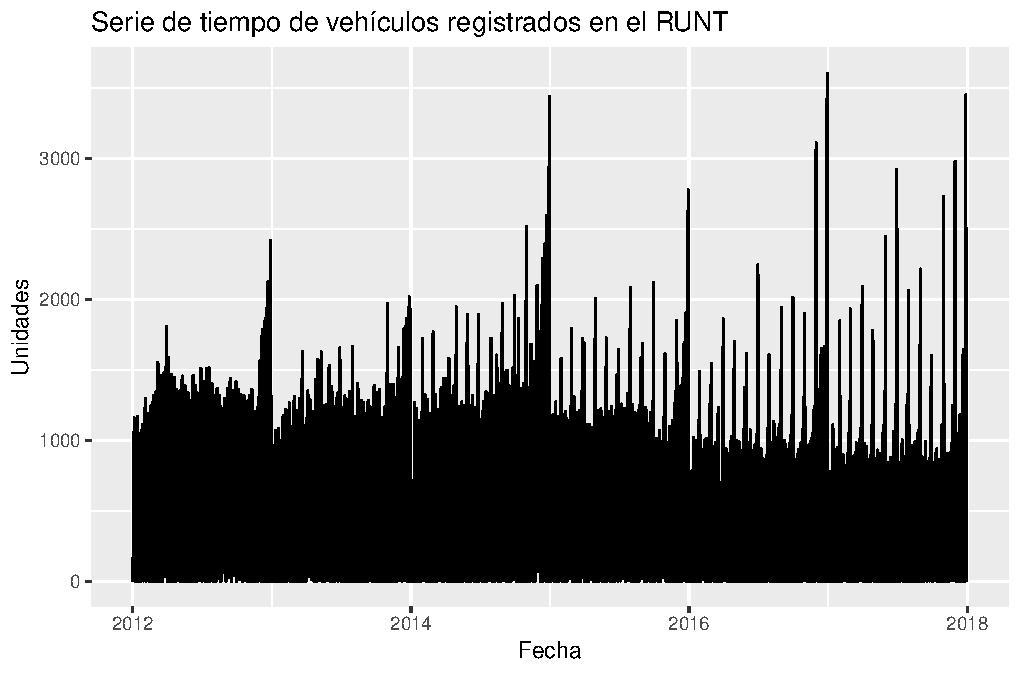
\includegraphics{serie1.pdf}
	\caption{Serie de tiempo del número de vehículos registrados en el RUNT desde el año 2012 hasta 2018}
\end{figure}

\noindent Se descarto trabajar el modelamiento de series de tiempo para poder hace el análisis de regresión haciendo uso de más variables predictoras sobre todo de tipo económico que representan significancia para el fenómeno analizado.
%% graifoco de dispercion de la variable respuest en funcion del tiempo 
\begin{figure}[H]
    \centering
	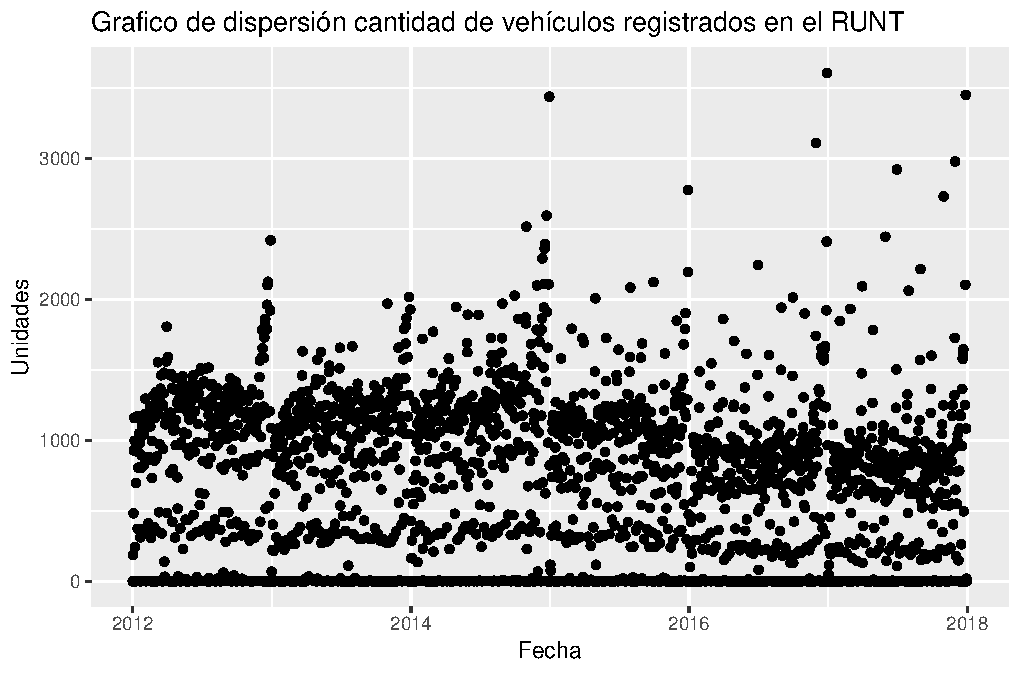
\includegraphics{xxx.pdf}
	\caption{Dispersión de la variable respuesta en función del tiempo}
\end{figure}
\begin{figure}[H]
    \centering
	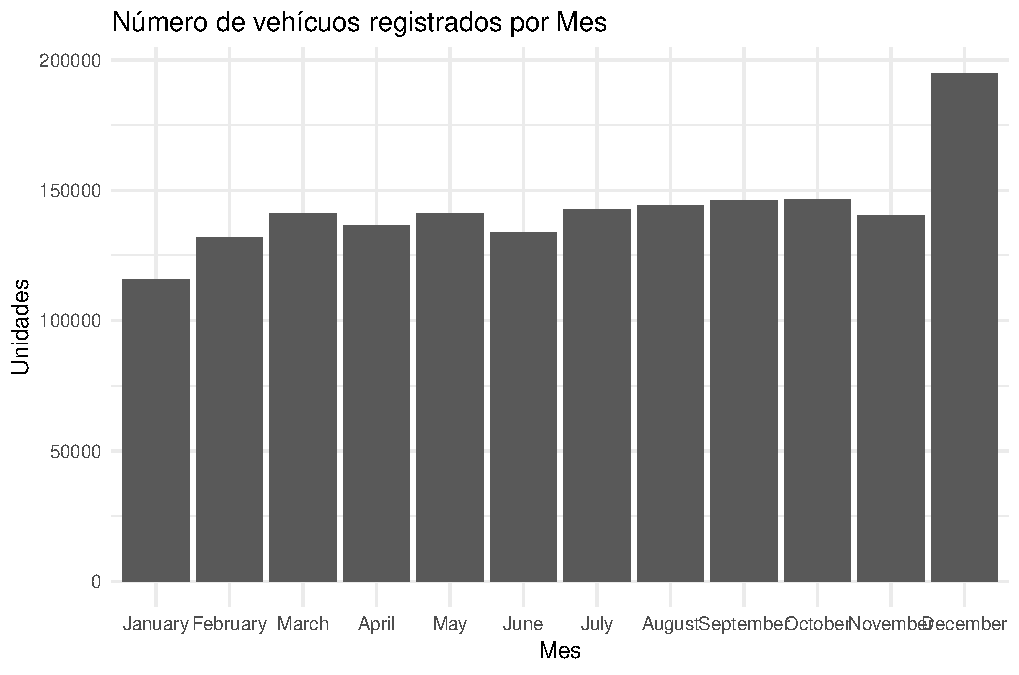
\includegraphics{pormes.pdf}
	\caption{Numero de vehículos registrados por mes}
\end{figure}
\noindent
Se puede notar en la Figura 3 el que el mes de diciembre es donde más se registran vehículos en el RUNT, posiblemente por las festividades de final de año.
\begin{figure}[H]
    \centering
	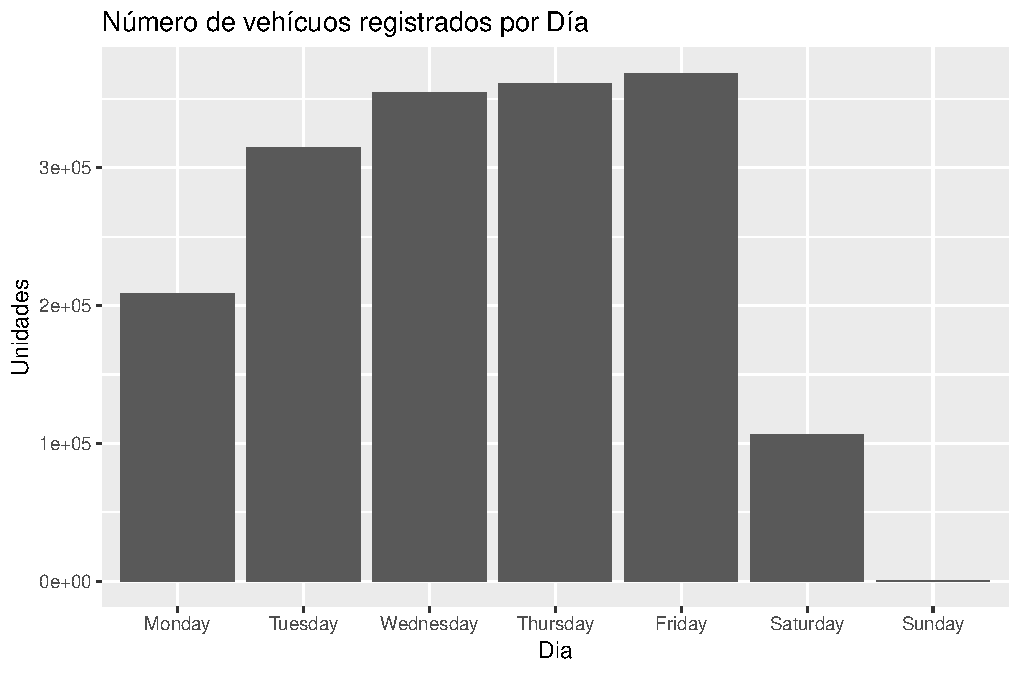
\includegraphics{pordia.pdf}
	\caption{Numero de vehículos registrados por Día}
\end{figure}
\noindent
\noindent
Es clave notar que el día domingo no se registran o se registran muy pocos vehículos en el RUNT por ende la variable respuesta tiene muchos ceros correspondientes al día domingo.
\\
\\
\noindent A continuación en la Figura 5 se muestra una matriz de dispersión para las variables cualitativas de la base de datos.
\begin{figure}[H]
   	\centering
	\includegraphics{descriptivo22.pdf}
	\caption{Matriz de dispersión múltiple con correlación para la variables cualitativas}
\end{figure}




% modelamiento estadistico ----------------------------

\subsection{Modelamiento estadístico}
\subsubsection{Modelo de regresion lineal múltiple}
\noindent Se partió de las siguientes variables recopiladas de distintas fuentes para construir el modelo.

\begin{table}[H]
\caption{\small{Variables en la base de datos y su descripción}}
\begin{tabular}{@{}llll@{}}
\toprule
Variable & Descripción & Variable & Descripción \\ \midrule
Año & (Variable cuantitativa) & TGP & Tasa Global de Participación \\
Mes & (Variable categórica) & TO & Tasa de Ocupación \\
Día & (Variable categórica) & TD & Tasa de Desempleo \\
ICC & Indice de confianza del consumidor & Google{\_}Trends & Búsqueda en google trends top3 vehículos \\
TRM & Tasa representativa del mercado &  & \\
PET & \% de personas en edad de trabajar &  &  \\ \bottomrule
\end{tabular}
\end{table}
\noindent Se ajusto un modelo de regresión lineal múltiple haciendo uso de la función \texttt{lm()} del software estadístico \textbf{R} y se obtuvieron los siguientes resultados ver Tabla 3.


\begin{table}[h]
	\caption{\small{Resumen del modelo1}}
	\label{tabla1}
	\centering {\small
\begin{tabular}{@{}cccccc@{}}
\toprule
Modelo & MSE & R$^{2}$ & R$_{pseudo}^{2}$ & \rho_{y,\hat{y}} & AIC \\ \midrule
Modelo1 & 104773.1  & 0.65 & 0.65 & 0.80 & 31613.17\\ 
\bottomrule
\end{tabular}}
\end{table}
\noindent Existe una buena correlación entre los valores reales y los valores ajustados (0.80), además el coeficiente de determinación indica que aproximadamente el 65{\%} de la variabilidad de los registros de vehículos en el RUNT es explicada por el modelo1
\\

\noindent Del modelo se calculó el pseudo coeficiente de determinación como sigue:
\\
\begin{equation}
    { R }^{ 2 }_{pseudo}=1-\frac { \sum _{ i=1 }^{ n }{ { ({ y }_{ i }-{ \hat { y }  }_{ i }) }^{ 2 } }  }{ \sum _{ i=1 }^{ n }{ { ({ y }_{ i }-{ \bar { y }  }) }^{ 2 } }  }  = 0.6532582
\end{equation}

\noindent Manejando un nivel de significancia del 5{\%}
las siguientes variables son relevantes para el modelo (solo se muestran las variables que resultaron significativas)


\begin{table}[H]
\caption{\small{Resumen del modelo1 estimado y valor-p}}
	\label{tabla1}
	\centering {\small
\begin{tabular}{@{}ccc@{}}
\toprule
Variable    & Estimado   & Valor-P         \\ \midrule
Año         & -2.190e$^{+02}$ & 0.0137         \\
MesDecember & 1.451e$^{+02}$  & 0.0167         \\
MesFebruary & 9.897e$^{+01}$  & 0.0202         \\
MesJune     & -8.175e$^{+01}$ & 0.02935         \\
MesNovember & -1.150e$^{+02}$ & 0.0252         \\
DiaMonday   & -5.121e$^{+02}$ & \textless 2e$^{-16}$ \\
DiaSaturday & -8.383e$^{+02}$ & \textless 2e$^{-16}$ \\
DiaSunday   & -1.175e$^{+03}$ & \textless 2e$^{-16}$ \\
DiaTuesday  & -1.173e$^{+02}$ & 3.65e$^{-11}$        \\
TRM{\_}Promedio & -8.099e$^{-01}$ & 0.05         \\
PET         & 9.886e$^{+03}$  & 0.0243         \\ 
Google{\_}Trends & 1.691$^{+03}$  & 0.05         \\\bottomrule
\end{tabular}}
\end{table}
\noindent
\textbf{Nota:} puesto que existen factores de la variable (Mes) y de la variable (Dia) que resultaron ser significativos se toman para el modelo todos los factores de dichas variables a si sean significativos o no.
\\
\\


\paragraph{Selección de variables}:\\
\\
\noindent
Se procedió hacer un proceso de selección de variables haciendo uso de la función \texttt{stepAIC()} del paquete \textbf{MASS} con parámetro \texttt{direction="backward"} lo cual nos permite hacer la selección de variables evaluando el \textbf{criterio de información de Akaike (AIC)} que representa una medida de la calidad relativa de un modelo estadístico.
\\
\\
El criterio de información de Akaike se define como $AIC=2k-2ln(L)$ \\

\noindent
donde $k$ es el número de parámetros en el modelo estadístico , y $L$ es el máximo valor de la función de verosimilitud para el modelo estimado.
\\
\\
El objetivo se la selección de variables es minimizar el AIC, a continuación se muestra el resultado obtenido con la función \textbf{stepAIC()} para este modelo.
\\
\begin{table}[H]
\caption{\small{Resultado del proceso de selección de variables haciendo uso de la función \texttt{stepAIC()}}}
	\label{tabla1}
\begin{tabular}{@{}cc@{}}
\toprule
Variable seleccionada & Descripción                                                   \\ \midrule
Año                   & Variable cuantitativa                                         \\
Mes                   & Variable Categórica                                           \\
Día                   & Variable Categórica                                           \\
ICC                   & Indice de confianza del consumidor                            \\
TRM\_Promedio         & Tasa representativa del mercado (promedio mes)                \\
PET                   & Personas en edad de trabajar ({\%})                           \\
TGP                   & Tasa Global de Participación                                  \\
Google\_Trends        & Búsqueda Google (top 3 vehículos mas vendidos en Colombia) \\ \bottomrule
\end{tabular}
\end{table}

\textbf{Con criterio de información de Akaike (AIC) = 25387.68}










\subsubsection{Modelo usando metodología Gamlss}

\noindent
Cuando se usa el modelo de regresión estándar se encuentran que muchas de las suposiciones en las que se basa rara vez se cumplen, El aprendizaje a partir de los datos requiere marcos de aprendizaje estadísticos que desafíen las suposiciones habituales de que la variable de respuesta tiene una distribución normal, con su media expresada como la suma de funciones lineales de las variables explicativas, y una varianza constante.
GAMLSS permite suponer una distribución paramétrica para la variable de respuesta y los parámetros de esta distribución pueden variar de acuerdo con las variables explicativas como funciones lineales, no lineales o funciones suaves de estas. Rigby, B.; Stasinopoulos, E (2005).
\\
\\
\textbf{Gamlss} permite suponer una distribución paramétrica para la variable de respuesta y los parámetros de esta distribución pueden variar de acuerdo con las variables explicativas como funciones lineales, no lineales o funciones suaves de estas.
\\
\\
Sea $D(.)$ una función de distribución generica y sea  $\mu, \sigma, \nu ,\tau $, parámetros de la distribución usaualmente localización, escala, forma(asimetria) y forma (curtosis) respectivamente, se define el modelamiento con Gamlss como sigue: 
\begin{center}
\begin{equation*}
\begin{split} 
Y\overset { ind }{ \sim  } D(\mu ,\sigma ,\nu ,\tau )\\ { \eta  }_{ 1 }={ g }_{ 1 }(\eta )={X }_{ 1 }{ \beta  }_{ 1 }+{ s }_{ 11 }({ x }_{ 11 })+...+{ s }_{ 1{ J }_{ 1 } }({ x }_{ 1{ J }_{ 1 } })\\ { \eta  }_{ 2 }={ g }_{ 2 }(\eta )={X}_{ 2 }{ \beta  }_{ 2 }+{ s }_{ 21 }({ x }_{ 21 })+...+{ s }_{ 2{ J }_{ 2 } }({x}_{ 2{ J }_{ 2 } })\\ { \eta  }_{ 3 }={ g }_{ 3 }(\eta )={X}_{ 3 }{ \beta  }_{ 3 }+{ s }_{ 31 }({ x }_{ 31 })+...+{ s }_{ 3{ J }_{ 3 } }({ x }_{ 3{ J }_{ 3 } })\\ { \eta  }_{ 4 }={ g }_{ 4 }(\eta )={ X  }_{ 4 }{ \beta  }_{ 4 }+{ s }_{ 41 }({ x }_{ 41 })+...+{ s }_{ 4{ J }_{ 4 } }({ x }_{ 4{ J }_{ 4 } })
\end{split}
\end{equation*}
\end{center}
${ \eta  }_{ i }={ g }_{ i }(\eta )$ son funciones lineales o no lienales de los parámetros de la distribución. 
\\
\\
Siguiendo esta metodología se ajustó dos modelos \textbf{Gamlss} suponiendo la variable respuesta con distribución Poisson \texttt{PO()} para el modelo2 y distribución  Poisson inflada en cero  \texttt{ZIP()} para el modelo3 y haciendo uso de las variables seleccionadas con la con la función \texttt{stepAIC()} del paquetes \textbf{MASS} (ver sección 3.2.1) (ver Tabla 5), estas variables seleccionadas se usaron para modelar la media, un resumen del resultado se muestra a continuación en la Tabla 6 y Tabla 7. 

\begin{table}[H]
\caption{\small{Resumen del modelo2}}
\centering {\small
\begin{tabular}{@{}cccccccc@{}}
\toprule
Modelo  & MSE      & R$^{2}$   & R$_{pseudo}^{2}$ & $\rho_{y, \hat{y}}$  & AIC & cant. covariables & Distribución \\ \midrule
Modelo2 & 100815.3 & 0.66 & 0.66     & 0.81 &  323569.5   & 8                             & Poisson      \\ \bottomrule
\end{tabular}}
\end{table}

\begin{table}[H]
\caption{\small{Resumen del modelo3}}
\centering {\small
\begin{tabular}{@{}cccccccc@{}}
\toprule
Modelo  & MSE      & R$^{2}$   & R$_{pseudo}^{2}$ & $\rho_{y, \hat{y}}$  & AIC & cant. covariables & Distribución \\ \midrule
Modelo3 & 104882.5 & 0.66 & 0.65     & 0.81 & 185906.1    & 8                             & Poisson inflada en cero     \\ \bottomrule
\end{tabular}}
\end{table}






\subsection{Diagnóstico del Modelo}
\noindent
Para seleccionar el modelo adecuado se hizo una comparación de las estadísticas de resumen de los dos modelos ajustados y así seleccionar el mejor, el resumen se muestra en la tabla 8. 


\begin{table}[H]
\caption{\small{Resumen de los 3 modelos calculados}}
\begin{tabular}{@{}cccccccc@{}}
\toprule
Modelo  & MSE      & R2   & R2pseudo & rho  & AIC      & cant. covariables & Distribución            \\ \midrule
Modelo1 & 104773.1 & 0.65 & 0.65     & 0.80 & 31613.1  & 11                & Normal                  \\
Modelo2 & 100815.3 & 0.66 & 0.66     & 0.81 & 323569.5 & 8                 & Poisson                 \\
Modelo3 & 104882.5 & 0.66 & 0.65     & 0.81 & 185906.1 & 8                 & Poisson inflada en cero \\ \bottomrule
\end{tabular}
\end{table}
\noindent
Se decide optar por el modelo 2 dado su alto pseudo coeficiente de determinación y su bajo número de variables.
\\
\\
A continuación, se muestra el gráfico de validación del Modelo2

\begin{figure}[H]
	\centering
	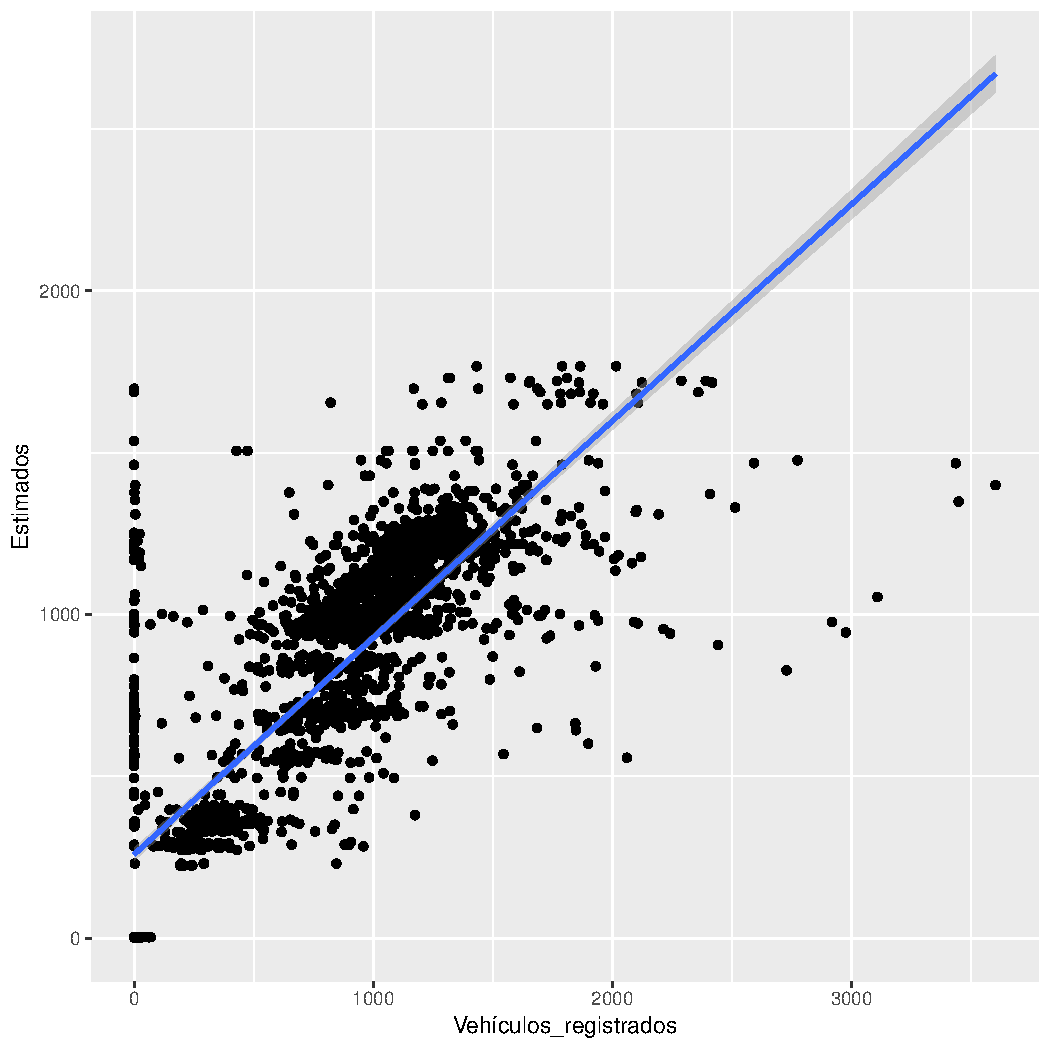
\includegraphics{chicharra33.pdf}
	\caption{Gráfico de  validacion del Modelo2}
\end{figure}
 
%***-----------------------------------------CONCLUCIONES--------------------------------------------------
\section{Conclusiones}
\noindent
Si se posee información real sobre una variable (en éste caso vehículos registrados en el RUNT, es posible encontrar variables explicativas de diversas fuentes de información real con las que se puede hacer un eficiente modelo predictivo, aún si inicialmente no se tenía ninguna variable explicativa.
\\
\\
Se encuentra que a partir de las variables de tipo económico y usando herramientas tecnológicas como google trends es posible modelar claramente el comportamiento del número de vehículos que se registran en el RUNT así poder implementar muy buenos modelos predictivos y dar solución a las necesidades que se demandan.





%***----------------------------------------APLICACION WEB--------------------------------------------
\section{Aplicación web}
\noindent
\paragraph{Enlace a la aplicación web.}
https://colnalitycs.shinyapps.io/Colnalitycs/
\begin{figure}[H]
	\centering
	
\includegraphics{qr_img.png}
	\caption{Código QR enlace a la aplicación web}
\end{figure}

\noindent
\paragraph{Enlace al video promocional} https://www.youtube.com/watch?v=VnDZXcw8xu4&feature=youtu.be



%***----------------------------------------REFERENCIAS--------------------------------------------
\section{Referencias}
\noindent

\begin{description}


\item[Rigby, B.; Stasinopoulos, E] (2005).
Generalized additive
models for location scale and shape. Applied Statistics

\item[Tasa de cambio del peso colombiano (TRM)]  recuperado de http://www.banrep.gov.co/es/trm


\item[Población Económicamente Activa]
recupeado de:\\
http://www.icesi.edu.co/cienfi/images/stories/pdf/glosario/poblacion-economicamente-activa.pdf (2018)


\item[RStudio Team:] (2018).
Integrated Development for R. RStudio, Inc., Boston, MA URL http://www.rstudio.com/.  


\end{description}

\end{document}
